\section{From Clovis to Charlemagne}

Under Constantine’s rule, Rome became more Christian. Over the next few centuries, some significant leaders brought Christianity to most of Europe. Christmas day was significant in these events.

\begin{wrapfigure}{tr}{.35\textwidth}
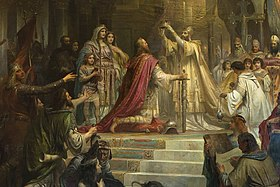
\includegraphics[scale=.5]{a20191225FromClovistoCharlemagne-img001.jpg} 
\end{wrapfigure}

\paragraph{Clovis (466-511)}
Clovis was the first of the 40 kings of France; he united all the Frankish tribes under one ruler. He was Baptized on Christmas Day 496, and three thousand of his companions converted with him.

\paragraph{King Ethelbert}
Pope Gregory the Great, having encountered some young Anglo-Saxons in a Roman slave market, was impressed by their beauty and blonde hair. He sent 40 Benedictine monks, under the leadership of Augustine of Canterbury (as he came to be known) to evangelize the English.

King Ethelbert embraced Christianity. Then he and 10 thousand citizens were baptized on Christmas day, year 597. The king’s baptism was the baptism of an entire people, who gladly followed their leader. From there, St Boniface and several monks set out to evangelize the Germans.

\paragraph{Charlemagne}
A century later, St Boniface was sent from England to evangelize the Germans. Progress was difficult, but after the felled the Donar Oak, without the gods subsequently striking him down, many pagans converted.

Charlemagne became King of the Franks in 768. As the Father of Europe, he re-united most of Roman Europe, even adding new lands to it. Charlemagne was not only a warrior, but the arts and sciences began to flourish again in Europe in the period called the Carolingian Renaissance. He valued learning and education. He encouraged the book publishing on a variety of topics, even founding a library at court. One of his favourite books was Augustine’s \emph{City of God}.

Charlemagne’s Coronation as Emperor of the Romans took place on Christmas day, 800 in Rome. The Roman people acclaimed:

\begin{quotex}
To Charles Augustus, crowned by God as great and pacific Emperor of the Romans, life and victory. 

\end{quotex}

Augustus was the same title claimed by Constantine, emphasizing the continuity between what was to be the Holy Roman Empire with the classical Roman Empire.

\flrightit{Posted on 2019-12-25 by Cologero}

\begin{center}* * *\end{center}

\begin{footnotesize}\begin{sffamily}

\texttt{Cologero on 2020-01-26 at 19:54 said: }

But the recovery of the Mediterranean West is prepared by the Empire of Charlemagne who, through a universal force characteristic of men who hold the spiritual and ethnic-blood heritage of the Romulean lineage, organizes Italy, France and part of Spain: it is strengthened with the supernationalist constitution of the Holy Roman Empire, continues its struggle through the maritime daring of the Maritime Republics of Genoa, Venice, Pisa and Amalfi. \flright{\textsc{Massimo Scaligero}, \textit{La Razza di Roma}}

\hfill
\end{sffamily}\end{footnotesize}